\documentclass[11pt,a4paper]{article}
\author{TalentSprint}
\date{}
\usepackage{verbatim}
\usepackage{fancyhdr}           % For header and footer
\usepackage{multicol}
\usepackage{colortbl}           % For coloured tables
\usepackage{setspace}           % For line height
\usepackage{seqsplit}           % Splits long words.
\usepackage{amsmath} 
\usepackage{graphicx}
\usepackage{array}
\usepackage{enumitem}
\usepackage{xcolor}
\usepackage[tikz]{bclogo}
\usepackage{textcomp}
\usepackage{listings}
\lstset{language=python,numbers=left,numberstyle=\tiny,numbersep=10pt,showstringspaces=false}

\headheight=14pt
\lhead{\nouppercase{}}
\rhead{\nouppercase{\leftmark}}

\newcommand*\lstinputpath[1]{\lstset{inputpath=#1}}
\lstinputpath{../Code/}
\graphicspath{{../Images/} {../ScreenShots/}}

\setcounter{tocdepth}{1}
\setlength\parindent{0pt}
\parskip=4pt
\newcommand{\Code}[1]{\textbf{\texttt{#1}}}

% Lengths and widths
\addtolength{\textwidth}{5cm}
\addtolength{\hoffset}{-1cm}
\setlength{\headsep}{-12pt} % Reduce space between header and content
\setlength{\headheight}{85pt} % If less, LaTeX automatically increases it
\renewcommand{\footrulewidth}{2pt} % Remove footer line
\renewcommand{\headrulewidth}{1pt} % Remove header line
\renewcommand{\seqinsert}{\ifmmode\allowbreak\else\-\fi} % Hyphens in seqsplit
% This two commands together give roughly
% the right line height in the tables
\renewcommand{\arraystretch}{1.3}
\onehalfspacing

% Commands
\newcommand{\SetRowColor}[1]{\noalign{\gdef\RowColorName{#1}}\rowcolor{\RowColorName}} % Shortcut for row colour
\newcommand{\mymulticolumn}[3]{\multicolumn{#1}{>{\columncolor{white}}#2}{#3}} % For coloured multi-cols
\newcolumntype{x}[1]{>{\raggedright}p{#1}} % New column types for ragged-right paragraph columns
\newcommand{\tn}{\tabularnewline} % Required as custom column type in use

% Font and Colours
\definecolor{HeadBackground}{HTML}{333333}
\definecolor{FootBackground}{HTML}{666666}
\definecolor{TextColor}{HTML}{333333}
\definecolor{DarkBackground}{HTML}{6B8E23} %{FD1AA8}
\definecolor{LightBackground}{HTML}{E8FED8} %D3FDC8
\definecolor{tit}{HTML}{FF6600}
\renewcommand{\familydefault}{\sfdefault}
\color{TextColor}
 \headsep = 25pt
% Header and Footer
\pagestyle{fancy}
\usepackage[headheight=110pt]{geometry}
\fancyhf{}% Clear header/footer

\fancyhead[r]{
\includegraphics[width = 4cm, height = 2cm]{TS-Logo.png}\hspace{0cm}}

%=================================TITLE=====================================
\fancyhead[l]{\Large{\bf{\textcolor{tit}{\textrm{Strings}}}}}
%===========================================================================

\renewcommand{\headrulewidth}{0.4pt}% Default \headrulewidth is 0.4pt
\renewcommand{\footrulewidth}{0.4pt}% Default \footrulewidth is 0pt

\rfoot{Page \thepage}
\lfoot{COPYRIGHT \textcopyright TALENTSPRINT, 2015. ALL RIGHTS RESERVED.}

\begin{document}

%\chapter{Strings}
\section*{Strings in C}
In C we do not have a real string data type. We have to use different approach to store and handle strings. We use array of characters to store strings, with a convention that there is a special character (null) after the last character of the string in that array. In other words, a string in C language is actually a one-dimensional array of characters terminated by a null character -- denoted by `$\backslash$0'. 

The following declaration and initialization create a string consisting of the word ``Hello''. To hold the null character at the end of the array, the size of the character array containing the string \emph{must} be one more than the number of characters in the word ``Hello''.

\subsubsection*{Example}
The following are equivalent:

\lstinline!char greeting[6] = {`H', `e', `l', `l', `o', `\0'};!

 OR

\lstinline!char greeting[ ] = ``Hello'';!

The representation of the above string in memory is as shown.

\begin{table}[ht]
\centering
\begin{tabular}{|c|c|c|c|c|c|}\hline
H & e & l & l & o & `$\backslash$0'\\\hline
\end{tabular}
\end{table}

You do not have to place the null character at the end of a string constant. The C compiler automatically places the `$\backslash$0' at the end of the string. But if you initialize an array of characters you have to do it yourself.

Strings are declared in C in similar manner as arrays. Only difference is that, strings are always of \lstinline!char! type.

\subsubsection*{Declaration}
\lstinline!char string_name[size];!

For example, \lstinline!char str[5];! 

\begin{table}[ht]
\centering
\begin{tabular}{|c|c|c|c|c|c|}
str[0] & str[1] & str[2] & str[3] & str[4]\\\hline
& & & & \\\hline
\end{tabular}
\end{table}

Strings can also be declared using pointer: \lstinline!char* p;!

\subsubsection*{Initialization}

In C, string can be initialized in a number of ways.

\lstinline!char c[ ] = ``abcd'';! 

OR \lstinline!char c[5] = ``abcd'';! 

OR \lstinline! char c[ ] = {`a', `b', `c', `d', `\0'};! 

OR \lstinline!char c[5] = {`a', `b', `c', `d', `\0'};! 

OR \lstinline!const char* c = ``abcd'';!

\begin{table}[ht]
\centering
\begin{tabular}{|c|c|c|c|c|c|}\hline
 c[0] & c[1] & c[2] & c[3] & c[4]\\\hline
 a & b & c & d & `$\backslash$0' \\\hline
\end{tabular}
\end{table}

\subsection*{String Input-Output} 
Let us look at the code right away.
\lstinputlisting{Program-11-1.c}

\begin{figure}[ht]
\begin{center}
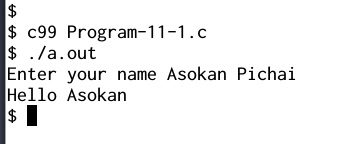
\includegraphics[scale=0.6]{Output-11-1.png}
\end{center}
\caption{String input}
\label{output-11-1}
\end{figure}

From the code and the execution, you can see two things:
\begin{enumerate}
  \item String variables read through \texttt{scanf()} can only take a word. It is because when white space is encountered, the \texttt{scanf()} function terminates. In the example, the second name is left in the buffer.
  \item The name of the string variable is its address; there is no need for \texttt{\&name}. This is true of arrays in general; if \texttt{p} is an array, \texttt{\&p[0] == p}.
\end{enumerate}

To write a string, we can use \texttt{printf()} function with format specifier ``\%s''. We saw the use in the previous code, where we printed the name.

There are two complementary functions, \texttt{gets()} and \texttt{puts()} for reading strings from the console and printing them respectively. They are also part of the standard input-output library.

\subsubsection*{Example} 

\lstinputlisting{Program-11-2.c}

\begin{figure}[ht]
\begin{center}
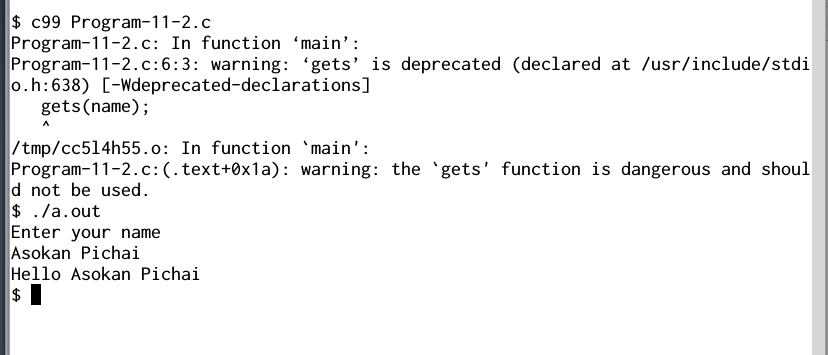
\includegraphics[scale=0.5]{Output-11-2.png}
\caption{Using gets()/puts()}
\label{output-11-2}
\end{center}
\end{figure}

\subsubsection*{Observations}
\begin{itemize}
\item \texttt{scanf()} ends reading when a space is encountered; when input is ``talent sprint'', \texttt{scanf()} reads only ``talent'' and when input is ``information technology'', \texttt{scanf()} reads only ``information''
\item To solve this problem we can use \texttt{gets()} input function -- but it is deprecated.
\item Both \texttt{scanf()} and \texttt{gets()} add the necessary `$\backslash$0' character at the end of the string.
\item Both \texttt{scanf()} and \texttt{gets()} cannot avoid the problems when the number of characters input is greater than the size of the string.
\item \texttt{puts()} adds a `$\backslash$n' to the end of the string. 
\item \texttt{printf()} is needed for combining and formatting output
\end{itemize}

We reproduce the relevant part of the \texttt{gets()} manual page to see why it is deprecated.

\begin{quote}
       Never use gets().  Because it is impossible to tell without knowing the data in advance how many characters gets() will read, and because gets() will continue to store characters past the end of the  buffer,  it  is  extremely  dangerous  to  use.  It has been used to break computer security.  Use fgets() instead.
\end{quote}

\subsection*{String Input}
We take a closer look at the options for string input; we will use \texttt{scanf()} to read a string with a space in it (it will give us trouble!). And then we will use the recommended \texttt{fgets()}. Please remember to use \texttt{scanf()} or \texttt{fgets()} depending on whether white space is expected to be part of the string or not. 
In both cases ensure that the size of the variables is sufficient. When calculating sizes do not forget that we need one more for the `$\backslash$0' character at the end. Thus ``Hello'' needs SIX character for storage and not five.

\subsubsection*{Examples}
\lstinputlisting{Program-11-3.c}
Note that we use an extra variable to capture the data left in the buffer by \texttt{scanf}. 

\begin{figure}[ht]

\begin{center}
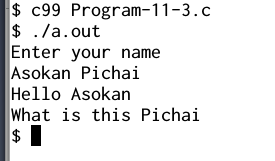
\includegraphics[scale=0.6]{Output-11-3.png}
\label{output-11-3}
\caption{scanf() trouble}
\end{center}
\end{figure}

Let us see how to use \texttt{fgets()}. The declaration is 

\lstinline!char* fgets(char* string, int size, FILE* stream)! 

Ignore the third parameter for now. Just remember that to replace \texttt{gets()} with \texttt{fgets()} you need to use \textbf{\texttt{stdin}} as the third parameter.
\lstinputlisting{Program-11-4.c}

\begin{figure}[ht]
\begin{center}
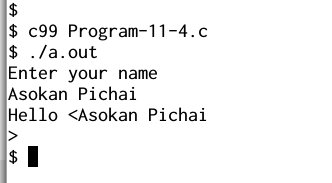
\includegraphics[scale=0.6]{Output-11-4.png}
\label{output-11-4}
\caption{Using fgets()}
\end{center}
\end{figure}

If you look at the output in Figure \ref{output-11-4}, you will notice a different problem: unlike \texttt{scanf()} and \texttt{gets()} the `$\backslash$n' character is now part of the input and that needs to be handled! Let us write a function which will use \texttt{fgets()} inside but remove the `$\backslash$n' character.

\lstinputlisting{Function-11-1.c}

\begin{figure}[ht]
\begin{center}
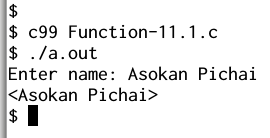
\includegraphics[scale=0.6]{Output-11-getstring.png}
\caption{getString() using fgets()}
\label{output-getString}
\end{center}
\end{figure}

\section*{String Handling Functions}
We can see the need to do the following:
\begin{itemize}
\item Finding the length of a string.
\item Comparing two strings.
\item Copying one string to another.
\item Joining two strings.
\end{itemize}

There are functions defined in \emph{\textless string.h \textgreater} header file to do these operations (and a few others). Let us look at these string handling functions.

\begin{description}
\item [strlen()] Returns the length of its string argument. As its declaration shows, it does \emph{not} modify the argument.

  \begin{itemize}
  \item \lstinline!int strlen(const char* str);! 
  \end{itemize}

\item [strcpy()] Copies the contents of the second argument to the first argument. As the declaration shows, the source is unmodified while of course destination is modified. Returns a pointer to the destination string.
  \begin{itemize}
    \item  \lstinline!char* strcpy(char* destination, const char* source);! 
  \end{itemize}

\item [strcat()] Concatenates -- joins -- two strings. It takes two arguments and appends contents of the second string to the first. Returns a pointer to the concatenated string.
  \begin{itemize}
    \item \lstinline!char* strcat(char* destination, const char* source);! 
  \end{itemize}

\item[strcmp()] Compares two strings and returns value 0, if the two strings are equal. Returns a +ve integer if the first string is greater than the second.  Returns -ve integer if first string is less than second. It does not modify either argument. \footnote{The comparison is based on lexical order. That is if the strings are sorted in dictionary order (that is characters with lower ASCII value come earlier than characters with greater ASCII value), and if str1 is earlier it returns a negative integer and if str1 is later it returns a positive integer.}  
  \begin{itemize}
    \item \lstinline!int strcmp(const char* str1, const char* str2);! 
  \end{itemize}
\end{description}

\subsubsection*{Example}

In this example we have used our own getString() function.
\lstinputlisting{Program-11-5.c}

\begin{figure}[ht]
\begin{center}
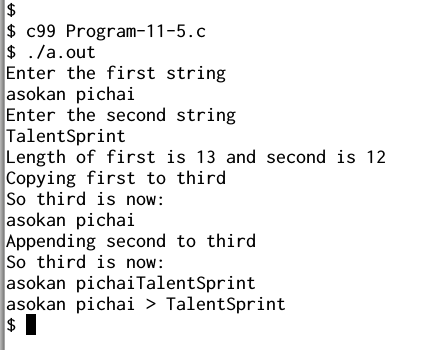
\includegraphics[scale=0.6]{Output-11-5.png}
\caption{String functions}
\label{output-11-5}
\end{center}
\end{figure}

\section*{Strings and Pointers}
Pointers and strings are closely related. We can treat them almost synonymously. Thus arrays of strings are easily dealt with as arrays of pointers.

\subsubsection*{Example}
\lstinputlisting{Program-11-6.c}

\begin{figure}[ht]

\begin{center}
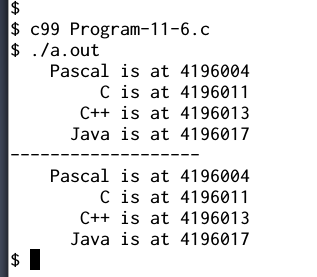
\includegraphics[scale=0.6]{Output-11-6.png}
\caption{Addresses and Contents}
\label{output-11-6}
\end{center}
\end{figure}

\subsection*{Important Points}
\begin{itemize}
\item All the string functions assume that sufficient memory is available. For example, if you say \texttt{strcat}($\alpha$, $\beta$), it is assumed that $\alpha$ was originally declared with a size $\geq$ \texttt{strlen}($\alpha$) + \texttt{strlen}($\beta$) + 1.
\item When pointers are used, its vital to ensure that overlapping strings are handled properly.
\end{itemize}
  
\section*{Arrays and Pointers}
What we said about strings and pointers holds for arrays and pointers too. We can say arrays and pointers are synonymous in terms of how they access memory. But, the important difference between them is that, a pointer variable can take different addresses as value whereas, in case of array it is fixed.

\lstinputlisting{Program-11-7.c}

\begin{figure}[ht]
\begin{center}
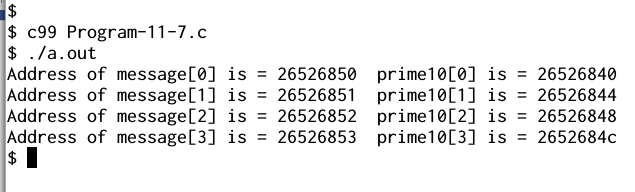
\includegraphics[scale=0.6]{Output-11-7.png}
\caption{Array element addresses}
\label{output-11-7}
\end{center}
\end{figure}

Notice the equal difference between consecutive elements of the arrays. As expected it is one byte between successive elements of a character array and 4 bytes for an integer array.

\emph{Note: You will get different starting addresses for the arrays.}

\subsubsection*{Pointer Arithmetic} 

Consider an array: \lstinline!int arr[4];!

The name of the array is synonymous with the address of the first element of the array. Here, address of first element of an array is \texttt{\&arr[0]}. 

\texttt{\&arr[0]} $\equiv$ \texttt{arr} and \texttt{arr[0]} $\equiv$ to \texttt{*arr)}.

\texttt{\&arr[1]} $\equiv$ \texttt{(arr + 1)} and \texttt{arr[1]} $\equiv$ to \texttt{*(arr + 1)}.

\texttt{\&arr[2]} $\equiv$ \texttt{(arr + 2)} and \texttt{arr[2]} $\equiv$ to \texttt{*(arr + 2)}.

\texttt{\&arr[3]} $\equiv$ \texttt{(arr + 3)} and \texttt{arr[3]} $\equiv$ to \texttt{*(arr + 3)}.


\begin{bclogo}[couleur=blue!5, arrondi=0.3, logo=\bcattention]{Note}
Now the most important point to remember is that adding 1 to a pointer makes it point to the next element; in this case it adds 4 bytes to the address.
\end{bclogo}

The next program will help us understand this point well.

\lstinputlisting{Program-11-8.c}

\begin{figure}[ht]
\begin{center}
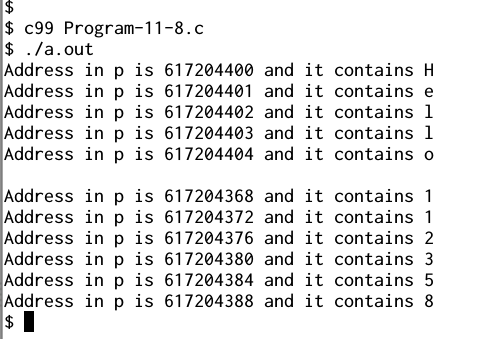
\includegraphics[scale=0.6]{Output-11-8.png}
\caption{Pointer increment}
\label{output-11-8}
\end{center}
\end{figure}

\section*{Dynamic Memory Allocation}
We noted that there should be sufficient memory allocated for holding the data, when pointers are used. When we declare an array variable, its size is allocated at compile time and cannot be changed. But using pointers and dynamic memory allocation, we can handle this problem.

There are 4 library functions under \emph{\textless stdlib.h \textgreater} for dynamic memory allocation.
\begin{enumerate}
\item malloc()
\item calloc()
\item realloc()
\item free()
\end{enumerate}

\subsection*{malloc() and free()}
The name malloc stands for ``memory allocation''. The function \texttt{malloc()} reserves a block of memory of specified size and returns a pointer of type \lstinline!void! which can be cast into pointer of any form. Its syntax is 

\texttt{ptr = (cast-type*) malloc(N);} 

Here, ptr is pointer of cast-type. The \texttt{malloc()} function returns a pointer to an area of memory whose size is \textbf{N}. If the memory available is insufficient, allocation fails and malloc returns \emph{NULL} pointer. 

\lstinline! int* ptr = (int*) malloc(100 * sizeof(int));! 

This statement declares a new pointer \texttt{ptr}, and allocates memory to store will 100 integer (400 bytes) and stores the address of the first byte of that block in \texttt{ptr}.

Please note that the memory is \emph{NOT} initialized. 

We need to call the function \texttt{free()} to release the memory which was allocated.

Let us write a program to sum the numbers entered by a user. If we use arrays to store the numbers, we have to assume that the user does not enter more than a given set of numbers.

We can remove that restriction, by allocating memory dynamically using \texttt{malloc()} function.

\lstinputlisting{Program-11-9.c}

\begin{figure}[ht]
\begin{center}
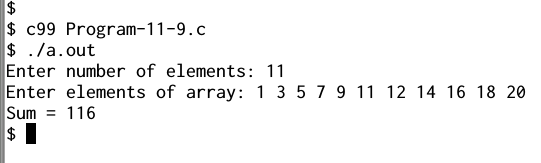
\includegraphics[scale=0.6]{Output-11-9.png}
\caption{malloc}
\label{output-11-9}
\end{center}
\end{figure}

\subsection*{calloc()}
The name calloc stands for ``contiguous allocation''. The major difference between \texttt{malloc()} and \texttt{calloc()} is that, \texttt{malloc()} allocates a single block of memory whereas \texttt{calloc()} allocates multiple blocks of memory each of the specified size and sets all the allocated memory to zero. 

\texttt{ptr = (cast-type*) calloc(n, element-size);}  This statement will allocate contiguous space in memory for an array of n elements. For example:

 \lstinline!ptr = (float*) calloc(25, sizeof(float));! allocates contiguous space in memory for an array of 25 elements each of size of \lstinline!float!, namely 4 bytes.

\subsection*{realloc()} 

If the previously allocated memory is insufficient or too much,  you can change using \texttt{realloc()}. 

\texttt{ptr = realloc(ptr, newsize);} Here, ptr is reallocated with size of newsize.

\begin{bclogo}[couleur=blue!5, arrondi=0.3, logo=\bcbombe]{WARNING}
The pointer given as argument to free() and realloc() must have the address as returned by an earlier malloc(), calloc() or realloc(). If that is not so, the results are undefined.
\end{bclogo}


\end{document}